%
% Slides for SLURM talk at User's meeting 
%                on
%            2003-04-08
%
% This presentation was built using a modified version of the
% ``prosper'' latex class and `alienglow' style 
% (See ./tex/prosper.cls and ./tex/PPRlinuxglow.sty)
%
% For the "interactive" PDF slides, uncomment the pdf option below
% to enable overlays. For printed slides, uncomment the ps option.
% 
\documentclass[%
letterpaper,
pdf,
%ps,
%nocolorBG,
%colorBG,
slideColor,
%slideBW,
%draft,
alienglow
]{prosper}

\usepackage{epsfig}

%
% Talk Title, SubTitle, etc.
%
\title{SLURM}
\subtitle{The Simple Linux Utility for \\ Resource Management}
\author{Mark A. Grondona}
\email{mgrondona@llnl.gov}
\disclaimer{LLNL internal use only}

%
% PPRalienglow.sty was directly modified to fit the two images below.
% If these are changed, you may need to adjust some values in that file.
%
\institution{
\epsfig{file=linux_llnl.eps,scale=.25}}
\Logo{
\epsfig{file=fry.eps,scale=.3}}

%
% Set default transition method. Valid methods are
% Replace, Split, Blinds, Box, Wipe, Dissolve, & Glitter
%
\DefaultTransition{Replace}

%
\begin{document}

%
% Make the title page
\maketitle

\begin{slide}{Overview}
\begin{itemize}
\item What is SLURM?
\item What SLURM is Not
\item SLURM Design Criteria
\item SLURM Components and Architecture
\item Simple Examples
\item SLURM and RMS Differences
\end{itemize}
\end{slide}

%
% Prepare a 5 overlay slide using the handy "itemstep" environment
% 
\overlays{5}{%
\begin{slide}{What is SLURM?}
\begin{itemstep}
  \item Simple resource manager:
  \begin{itemstep}
    \item Allocates access to resources (nodes)
    \item Distributes work to allocated resources.
    \item Manages conflicting requests for resources by maintaining a 
          simple queue of pending work.
  \end{itemstep}
  \item Open Source replacement for RMS
\end{itemstep}
\end{slide}}

%
\overlays{3}{%
\begin{slide}{What SLURM is Not}
\begin{itemstep}
  \item A sophisticated job scheduler. 
  \item A meta-batch system.
  \item A comprehensive cluster administration or monitoring package.
\end{itemstep}
\end{slide}}

%%
%%
\begin{slide}{SLURM Design Criteria}
\begin{itemize}
 \item Simple
 \item Efficient
 \item Scalable to clusters with thousands of nodes
 \item Fault Tolerant
 \item Secure
 \item Open Source
\end{itemize}
\end{slide}

%
% Prepare overlays using the onlySlide* command. Slides 2-5 will
% show the diagrams entities0-5.eps respectively. The onlySlide*
% environment deallocates the space taken by the slide contents.
%
\overlays{5}{%
\begin{slide}{SLURM Entities}
 \onlySlide*{1}{%
  \begin{itemize}
    \item Nodes
    \item Partitions
    \item Jobs
    \item Job Steps
  \end{itemize}}
 \begin{center}
  \onlySlide*{2}{\epsfig{file=entities0.eps,scale=0.5}}
  \onlySlide*{3}{\epsfig{file=entities1.eps,scale=0.5}}
  \onlySlide*{4}{\epsfig{file=entities2.eps,scale=0.5}}
  \onlySlide*{5}{\epsfig{file=entities3.eps,scale=0.5}}
  \onlyInPS{\epsfig{file=entities3.eps,scale=0.5}}
 \end{center}
\end{slide}}

%
%
\overlays{2}{%
\begin{slide}{SLURM Architecture}
\onlySlide*{1}{%
\begin{itemize}
 \item Two daemons
   \begin{itemize}
   \item {\tt slurmctld}: controller daemon
   \item {\tt slurmd}: compute node daemon
   \end{itemize}
 \item Five simple commands
   \begin{itemize}
    \item {\tt scontrol, sinfo, squeue, scancel, srun}
   \end{itemize}
\end{itemize}}
\onlySlide*{2}{%
  \begin{center}
  \epsfig{file=arch.eps,scale=0.3}
  \end{center}}
  \onlyInPS{\hfill \epsfig{file=arch.eps,scale=0.3} \hfill}
\end{slide}}

%
% Simple use of tabular environment.
%
\begin{slide}{User Commands}
\begin{tabular}{rc}
{\tt scontrol} & SLURM administration utility \\
{\tt sinfo}    & Partition and node state \\
{\tt squeue}   & Query job state \\
{\tt scancel}  & Cancel pending jobs \\
{\tt srun}     & Allocate resources and run job steps \\
\end{tabular}
\end{slide}


%
% Use of verbatim environment within a slide.
% The font size is shrunk to footnotesize and TeX's baselineskip is
% decreased by 20% because the default monospace font was so darn big.
%
\begin{slide}{Simple SLURM Examples}
\begin{itemize}
\item Basic interface very similar to RMS
\end{itemize}
\renewcommand{\baselinestretch}{0.8}
\footnotesize
\begin{verbatim}
grondo@dev0 ~ > sinfo
PARTITION  NODES STATE  CPUS MEMORY TMP_DISK NODES
------------------------------------------------------
debug         18 IDLE      2   2012    64324 dev[0-17]
grondo@dev0 ~ > srun -N4 hostname
dev0
dev1
dev2
dev3
grondo@dev0 ~ >
\end{verbatim}
\renewcommand{\baselinestretch}{1.0}
\end{slide}

%
%
\begin{slide}{Simple SLURM Examples}
\begin{itemize}
\item Killing an interactive job
\end{itemize}
\renewcommand{\baselinestretch}{0.8}
\footnotesize
\begin{verbatim}
grondo@dev0 ~ > srun -n8 sleep 30
srun: interrupt (one more within 1 sec to abort)
srun: task[0-7]: running
srun: sending Ctrl-C to job
srun: error: dev0: task[0-1]: Interrupt
srun: error: dev1: task[2-3]: Interrupt
srun: error: dev3: task[6-7]: Interrupt
srun: error: dev2: task[4-5]: Interrupt
grondo@dev0 ~ >
\end{verbatim}
\renewcommand{\baselinestretch}{1.0}
\end{slide}

%
%
\begin{slide}{Simple SLURM Examples}
\begin{itemize}
\item Killing a queued job
\end{itemize}
\renewcommand{\baselinestretch}{0.8}
\footnotesize
\begin{verbatim}
grondo@dev0 ~ > squeue
JobId Partition Name   User   St TimeLim Prio Nodes
   14 debug     sleep  grondo R     0:30 0.99 dev[0-3]
grondo@dev0 ~ > scancel 14
grondo@dev0 ~ > squeue
JobId Partition Name  User    St TimeLim Prio Nodes
grondo@dev0 ~ >
\end{verbatim}
\renewcommand{\baselinestretch}{1.0}
\end{slide}

%
%
\begin{slide}{SLURM and RMS Differences}
\raggedright
\begin{itemize}
\item SLURM infrastructure is much simpler 
  \begin{itemize}
  \item SLURM uses a simple configuration file not database
  \item Initially, no back-end database \\ 
        (future versions of SLURM may have this)
  \end{itemize}
\item SLURM Open Source and locally developed to fit our needs
\item Job submission and query will mostly be through DPCS, so no changes
      there
\end{itemize}
\end{slide}

%
%
\begin{slide}{prun vs. srun}
\raggedright
\begin{itemize}
\item Most used user command, {\tt srun}, very similar to RMS's {\tt prun}
      with minor differences:
  \begin{itemize}
  \item Basic options: -n,  -N, -c, -I, -O, -v are the same
  \item I/O redirection --  -e, -i, -o -- are similar
  \item Other options differ moderately to significantly
  \item Signal Handling in {\tt srun} slightly different
  \item We will try to offer a ``prun'' wrapper for {\tt srun} in early versions
  \end{itemize}
\end{itemize}
\end{slide}

%
\begin{slide}{Any Questions?}
\hfill \hfill \epsfig{file=slurm.eps,scale=0.5} \hfill
\end{slide}

\end{document}
